\documentclass[a4paper, 11pt]{article}
\usepackage[french]{babel}
\usepackage[utf8]{inputenc} 
\usepackage[T1]{fontenc}
\usepackage{multirow, multicol}
\usepackage{amsmath, amssymb, latexsym}
\usepackage{graphicx, epsfig,subfigure}
\usepackage[lined,boxed]{algorithm}
\usepackage{algorithmic}
\usepackage{rotate}
\usepackage{url}
\usepackage{setspace}
\usepackage{fancyhdr}
\usepackage{color}


\newtheorem{definition}{Definition}
\newtheorem{example}{Example}
\newtheorem{proposition}{Proposition}
\newtheorem{proof}{Proof}
\pagestyle{fancy}
\fancyhf{}
\newcommand{\univ}{
\epsfig{file = images/logoUni.png, height = 1.05cm}}
\lhead{\univ}
\rhead{\date{\today}}
\rfoot{Page \thepage}

\title{}
\author{CHAMPENOIS Brandon \textsc{G5B} \\ BONVARLET Bastien \textsc{G5B} \\ MASSON Joris \textsc{G5B} }

\begin{document}
\maketitle
\centerline{
\includegraphics[width = 7cm]{images/ecos.png}}
\tableofcontents
\newpage

\section{Rapide présentation / résumé du projet}
Notre projet est une simulation d'écosystème\\

\subsection*{Qu'est-ce qu'une simulation d'écosystème ?}
Tout d'abord qu'est-ce qu'une simulation d'écosystème ?\\
Alors une simulation d'écosystème c'est une simulation de vie, reprenant plusieurs critères comme :\\
La reproduction, chasse, "guerre", faim...\\

\subsection{Ce que fait notre simulation}
Notre simulation fait :\\
\newpage

\section{Qui a fait quoi ?}

Bonvarlet bastien :\\
Masson Joris : \\
Champenois Brandon : Le menu du jeu, le rapport latex, les sprites de chaque entités

\subsection{Résumé de ce qui a était fait durant les semaines du projet}

Bonvarlet Bastien :\\
\begin{enumerate}
\item Pour toutes les modifs pour la map et les bases graphiques et codes du log : A passer une dizaine d'heures sur les deux premières semaines.\\
\item Pour la gestion des déplacements de base : a peu près 1-2 heures en tout.\\
\item Pour la création du logo : a peu près 1-2 heures en tout.\\
\item Pour les animations : \\
\item Pour le sprite du lapin : (insérer figure du lapin)\\
\end{enumerate}
\newpage
Masson Joris : \\
\begin{enumerate}
\item Il a passé environ 15-20h sur l'alogorithme  A*.
\item Il a fait le beamer du "" au "".
\end{enumerate}
\newpage
Champenois Brandon : \\
\begin{enumerate}
\item Durant les 3 premières semaines a fait tout les sprites de notre simulation d'écosystème :\\
\item Après avoir récupérer le sprite de l'humain :
\\
\begin{figure*}[ht!]
 \centering
 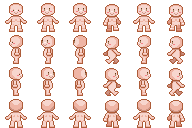
\includegraphics[width=0.5\linewidth]{images/human.png}
 \caption{sprite de l'humain}
 \label{fig::example::one}
\end{figure*} 
\\
\item A fait l'orc il lui suffisait juste de recolorer le sprite de l'humain :
\\ 
\begin{figure*}[ht!]
 \centering
 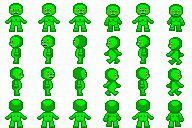
\includegraphics[width=0.5\linewidth]{images/orc.png}
 \caption{sprite de l'orc}
 \label{fig::example::one}
\end{figure*}
\\
Cela lui a pris 3-4 heures\\
\\
\item Il a donc ensuite fait des croquis pour les autres entités :
\\
\begin{figure*}[ht!]
  \begin{minipage}[c]{.5\linewidth}
   \centering
   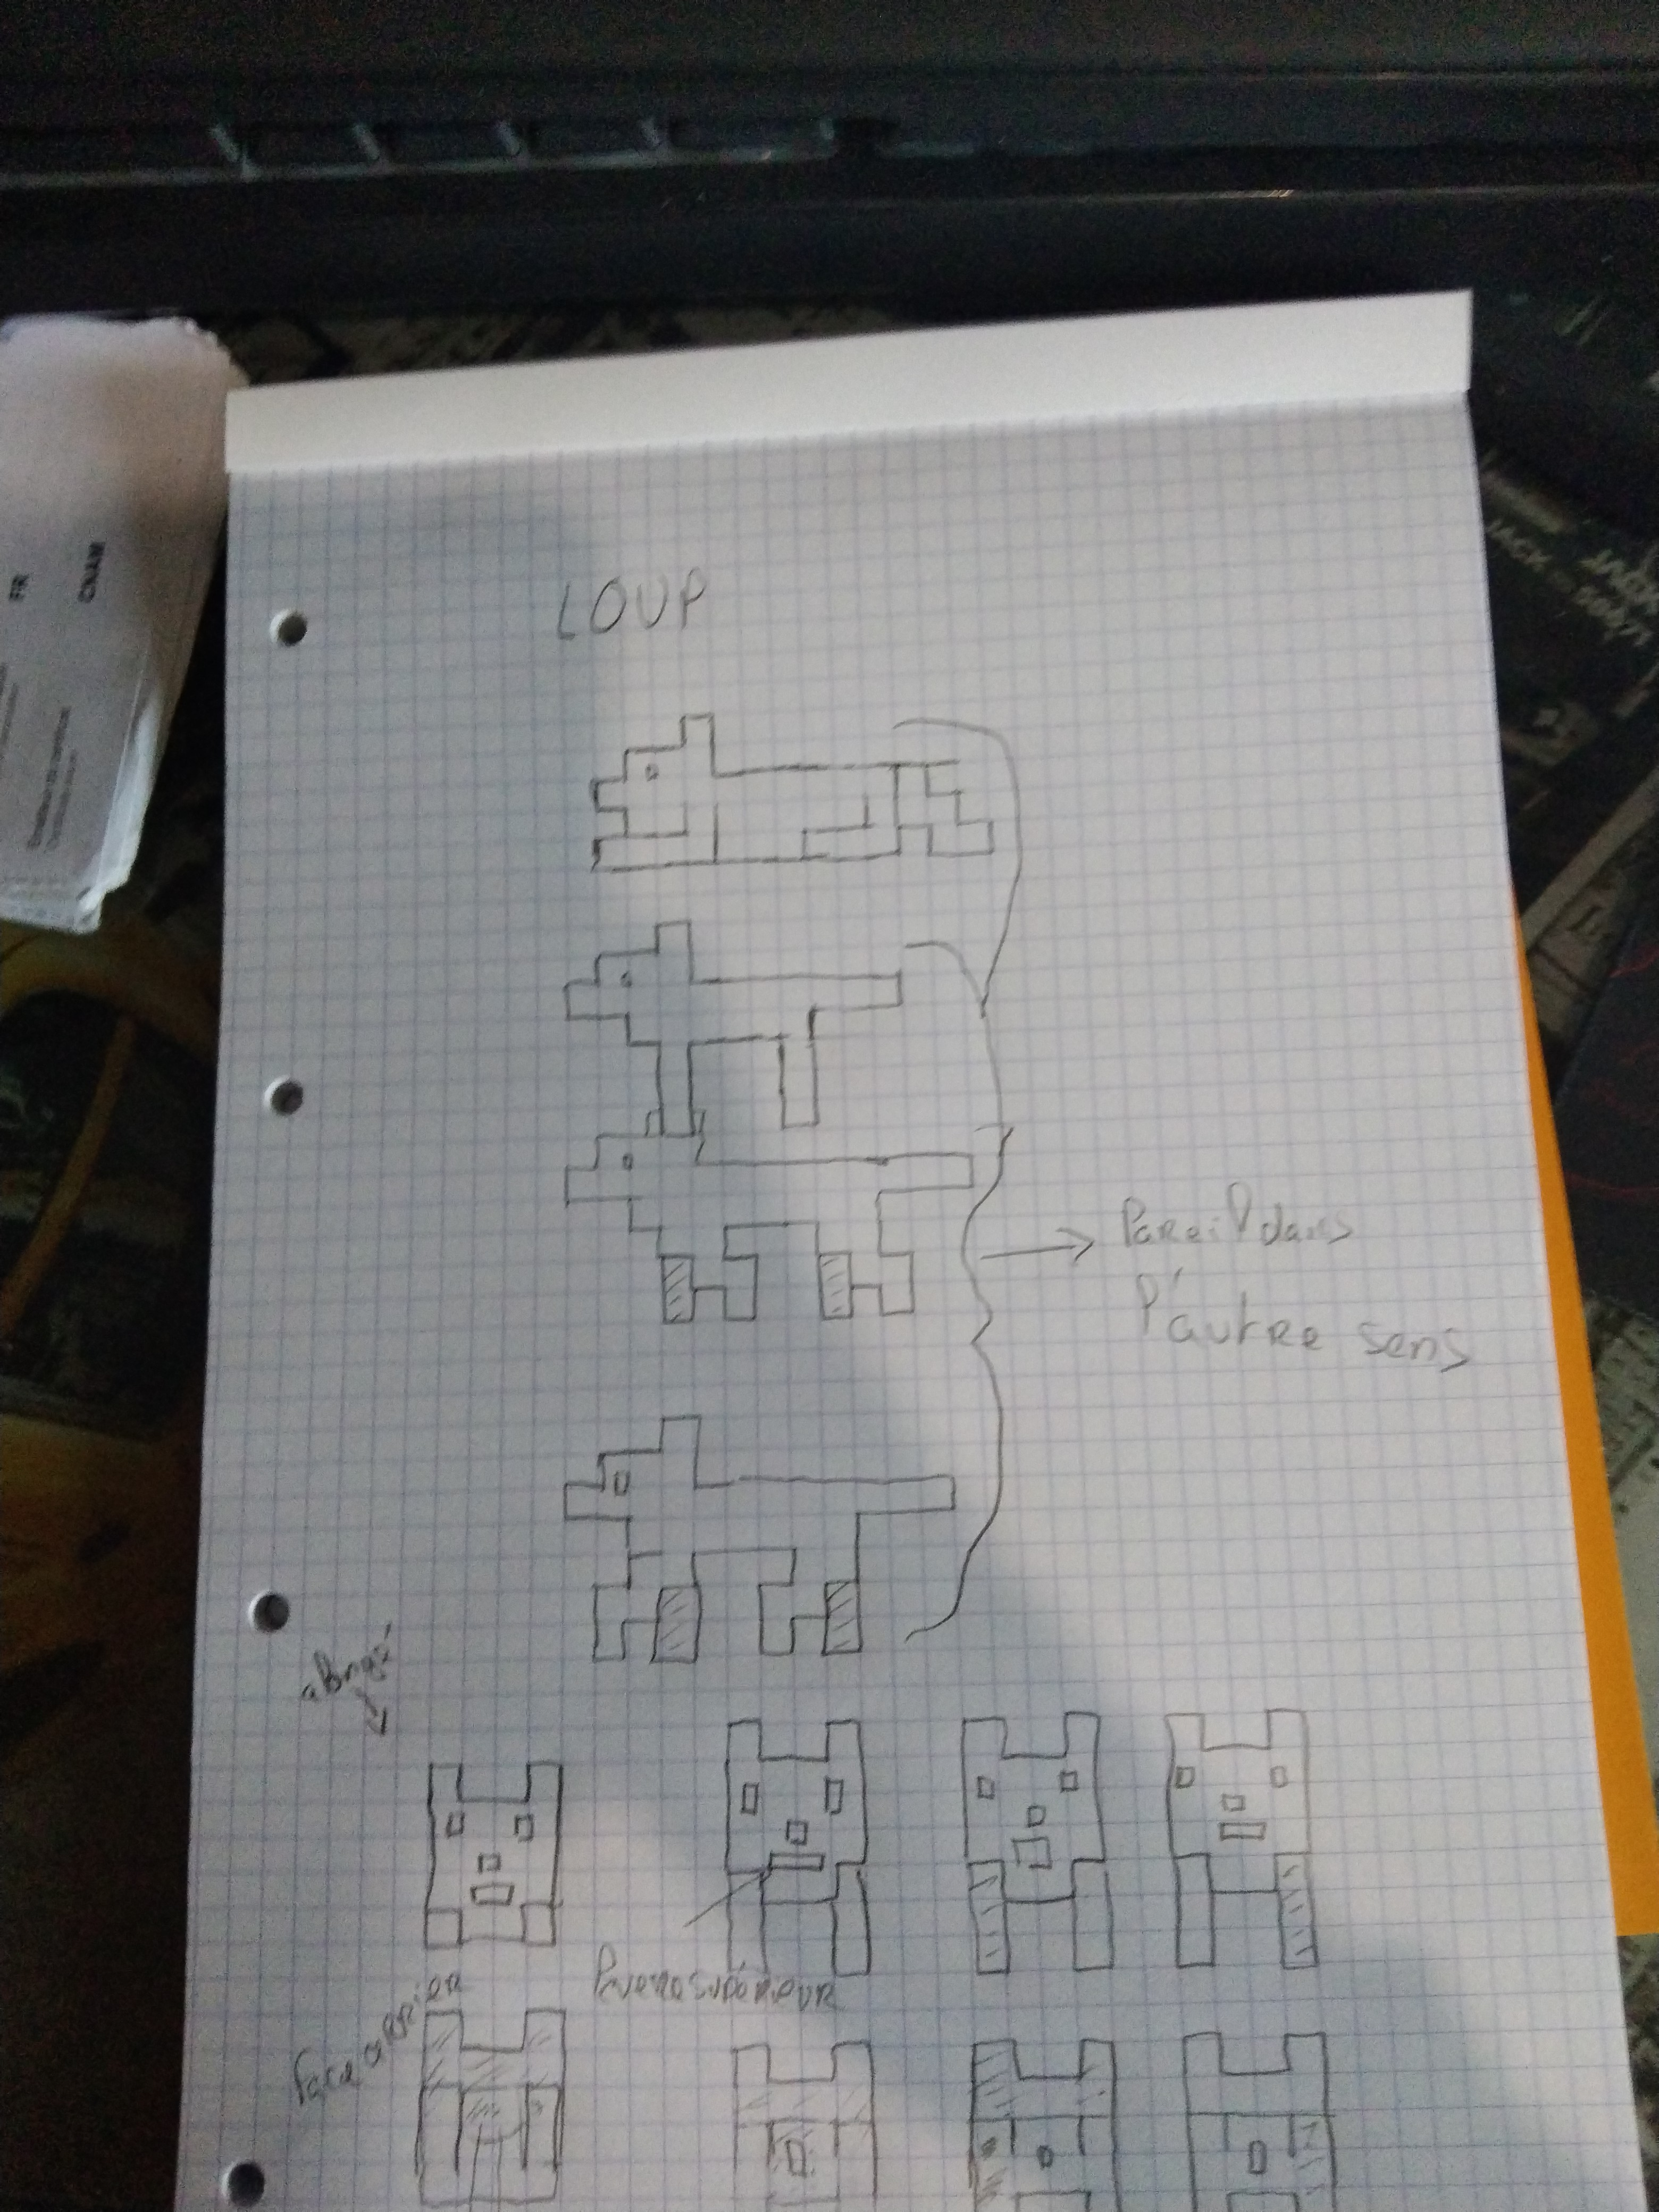
\includegraphics[width=\linewidth]{images/loup.jpg}
  \end{minipage} \hfill
  \begin{minipage}[c]{.5\linewidth}
   \centering
   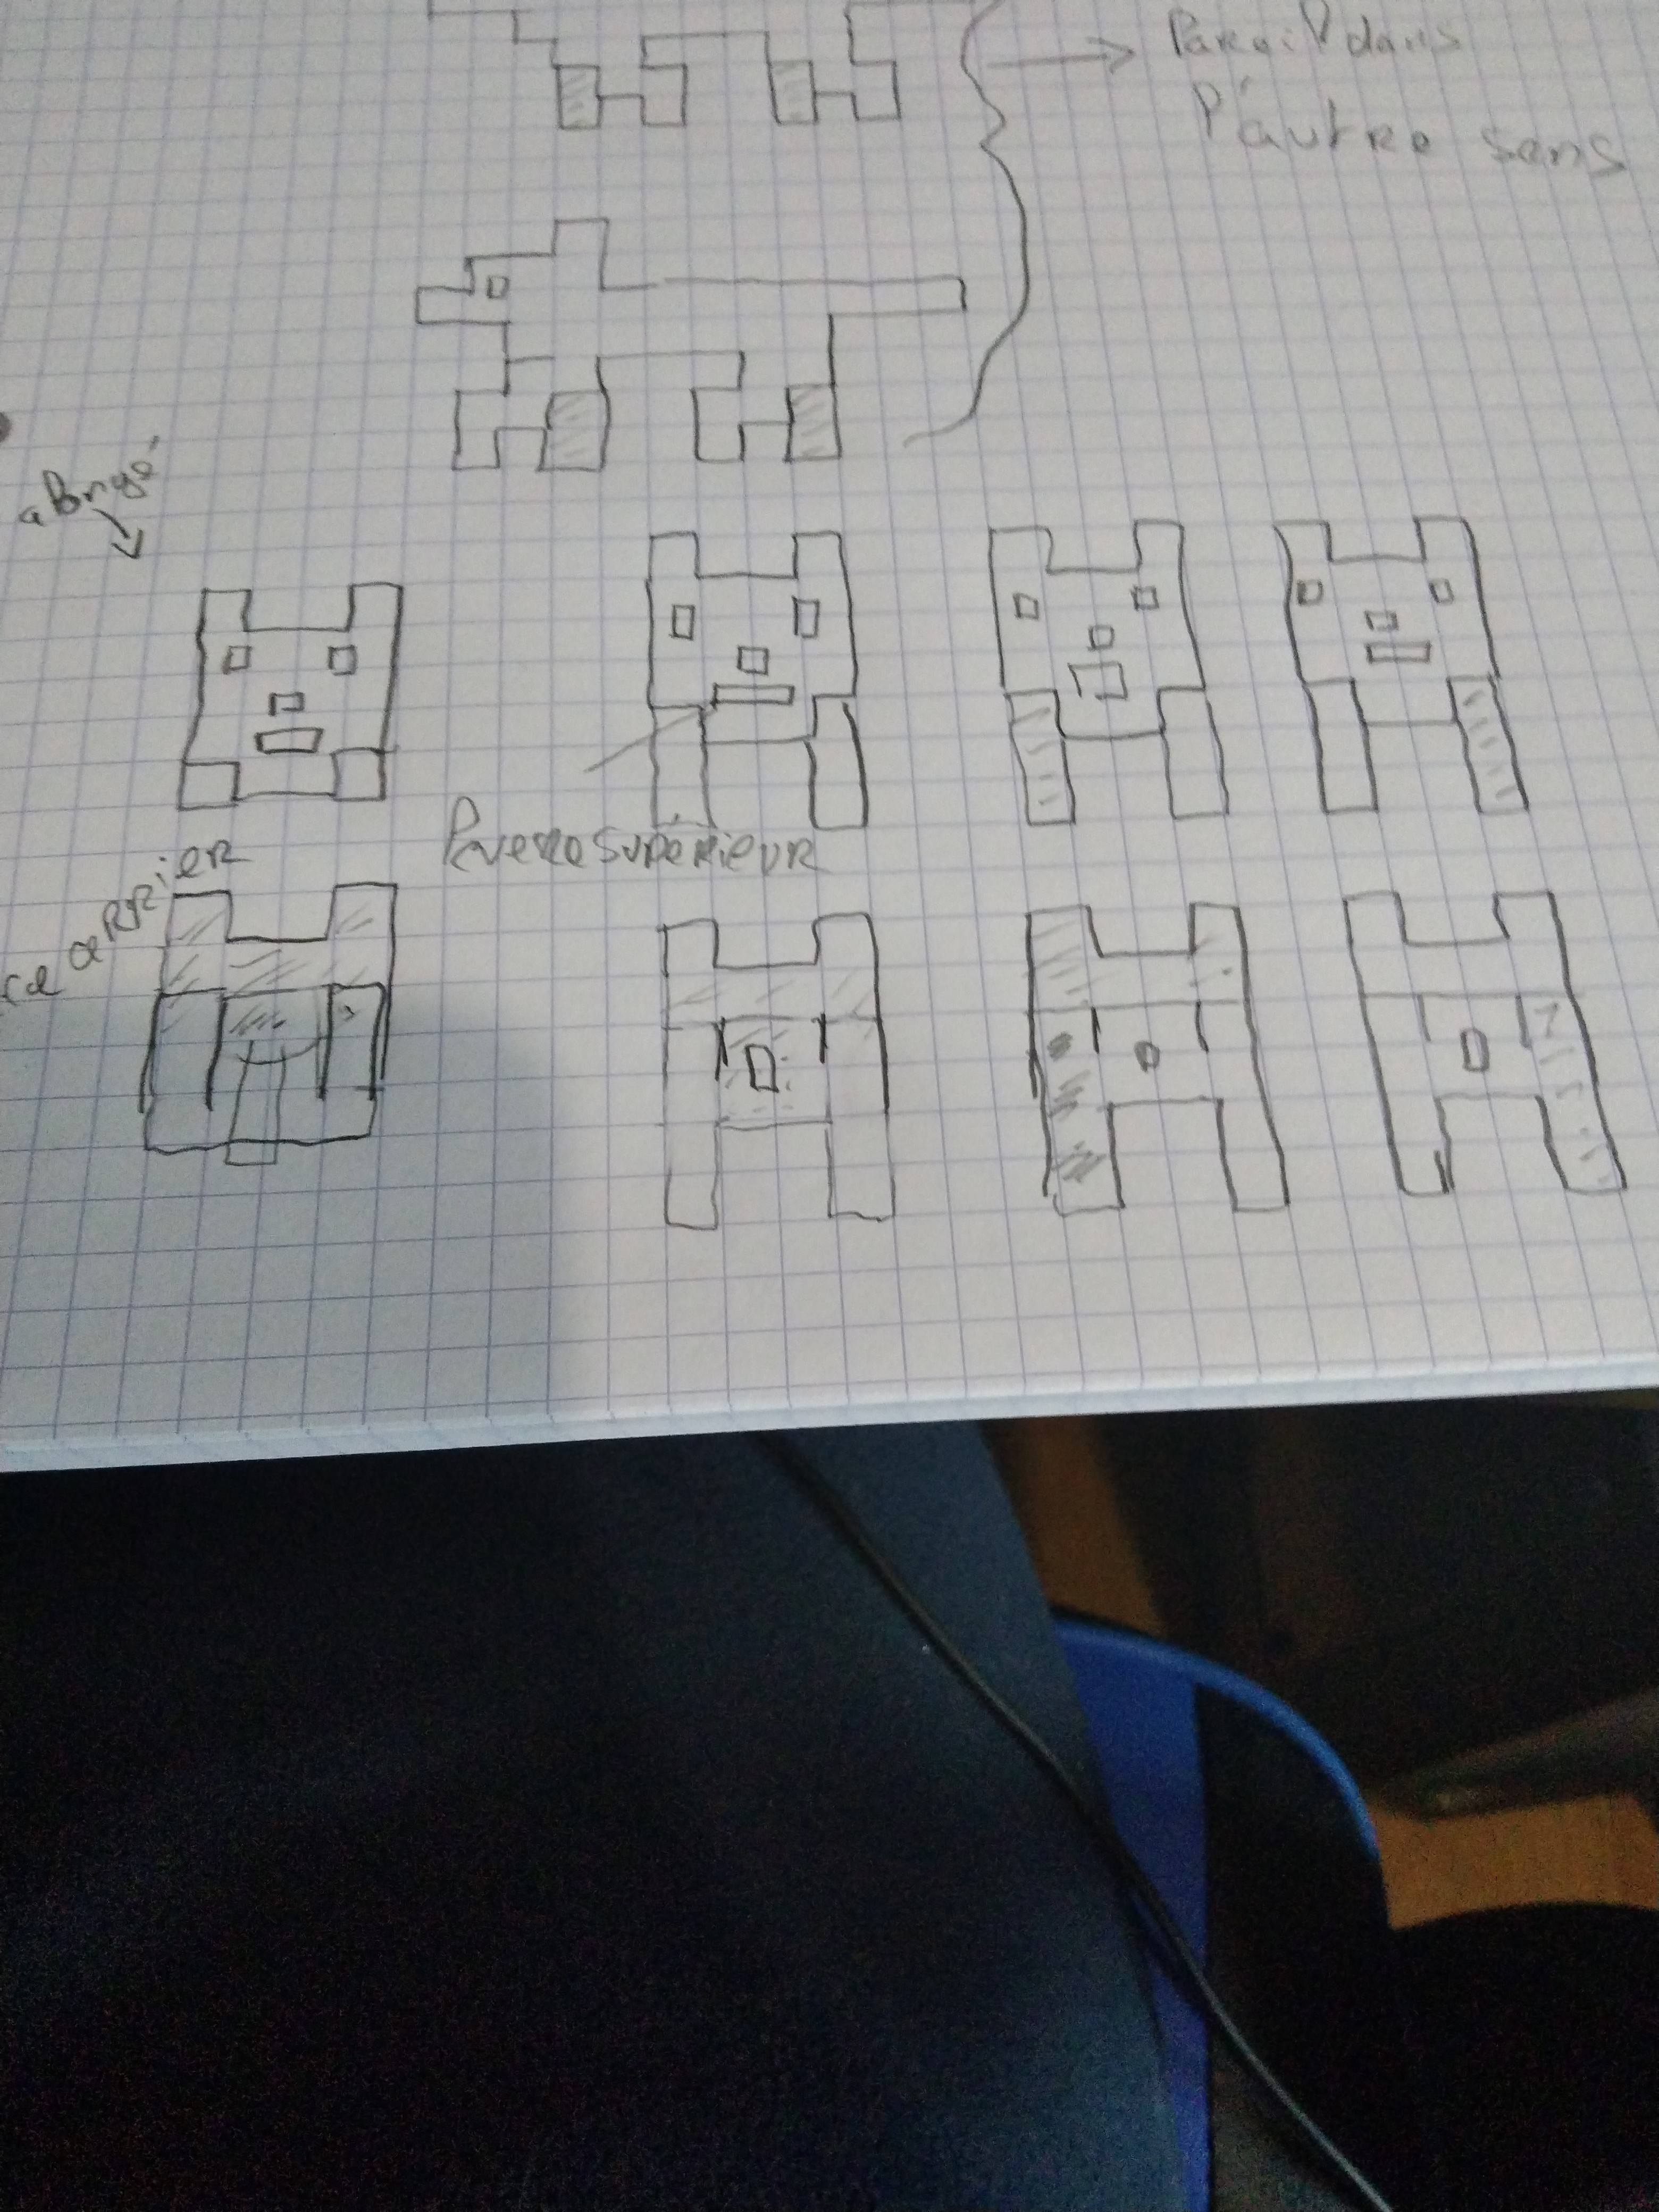
\includegraphics[width=\linewidth]{images/loup2.jpg}
  \end{minipage}
  \caption{(a) croquis du loup}
  \label{fig::example::two}
\end{figure*}
\\
\begin{figure*}[ht!]
 \centering
 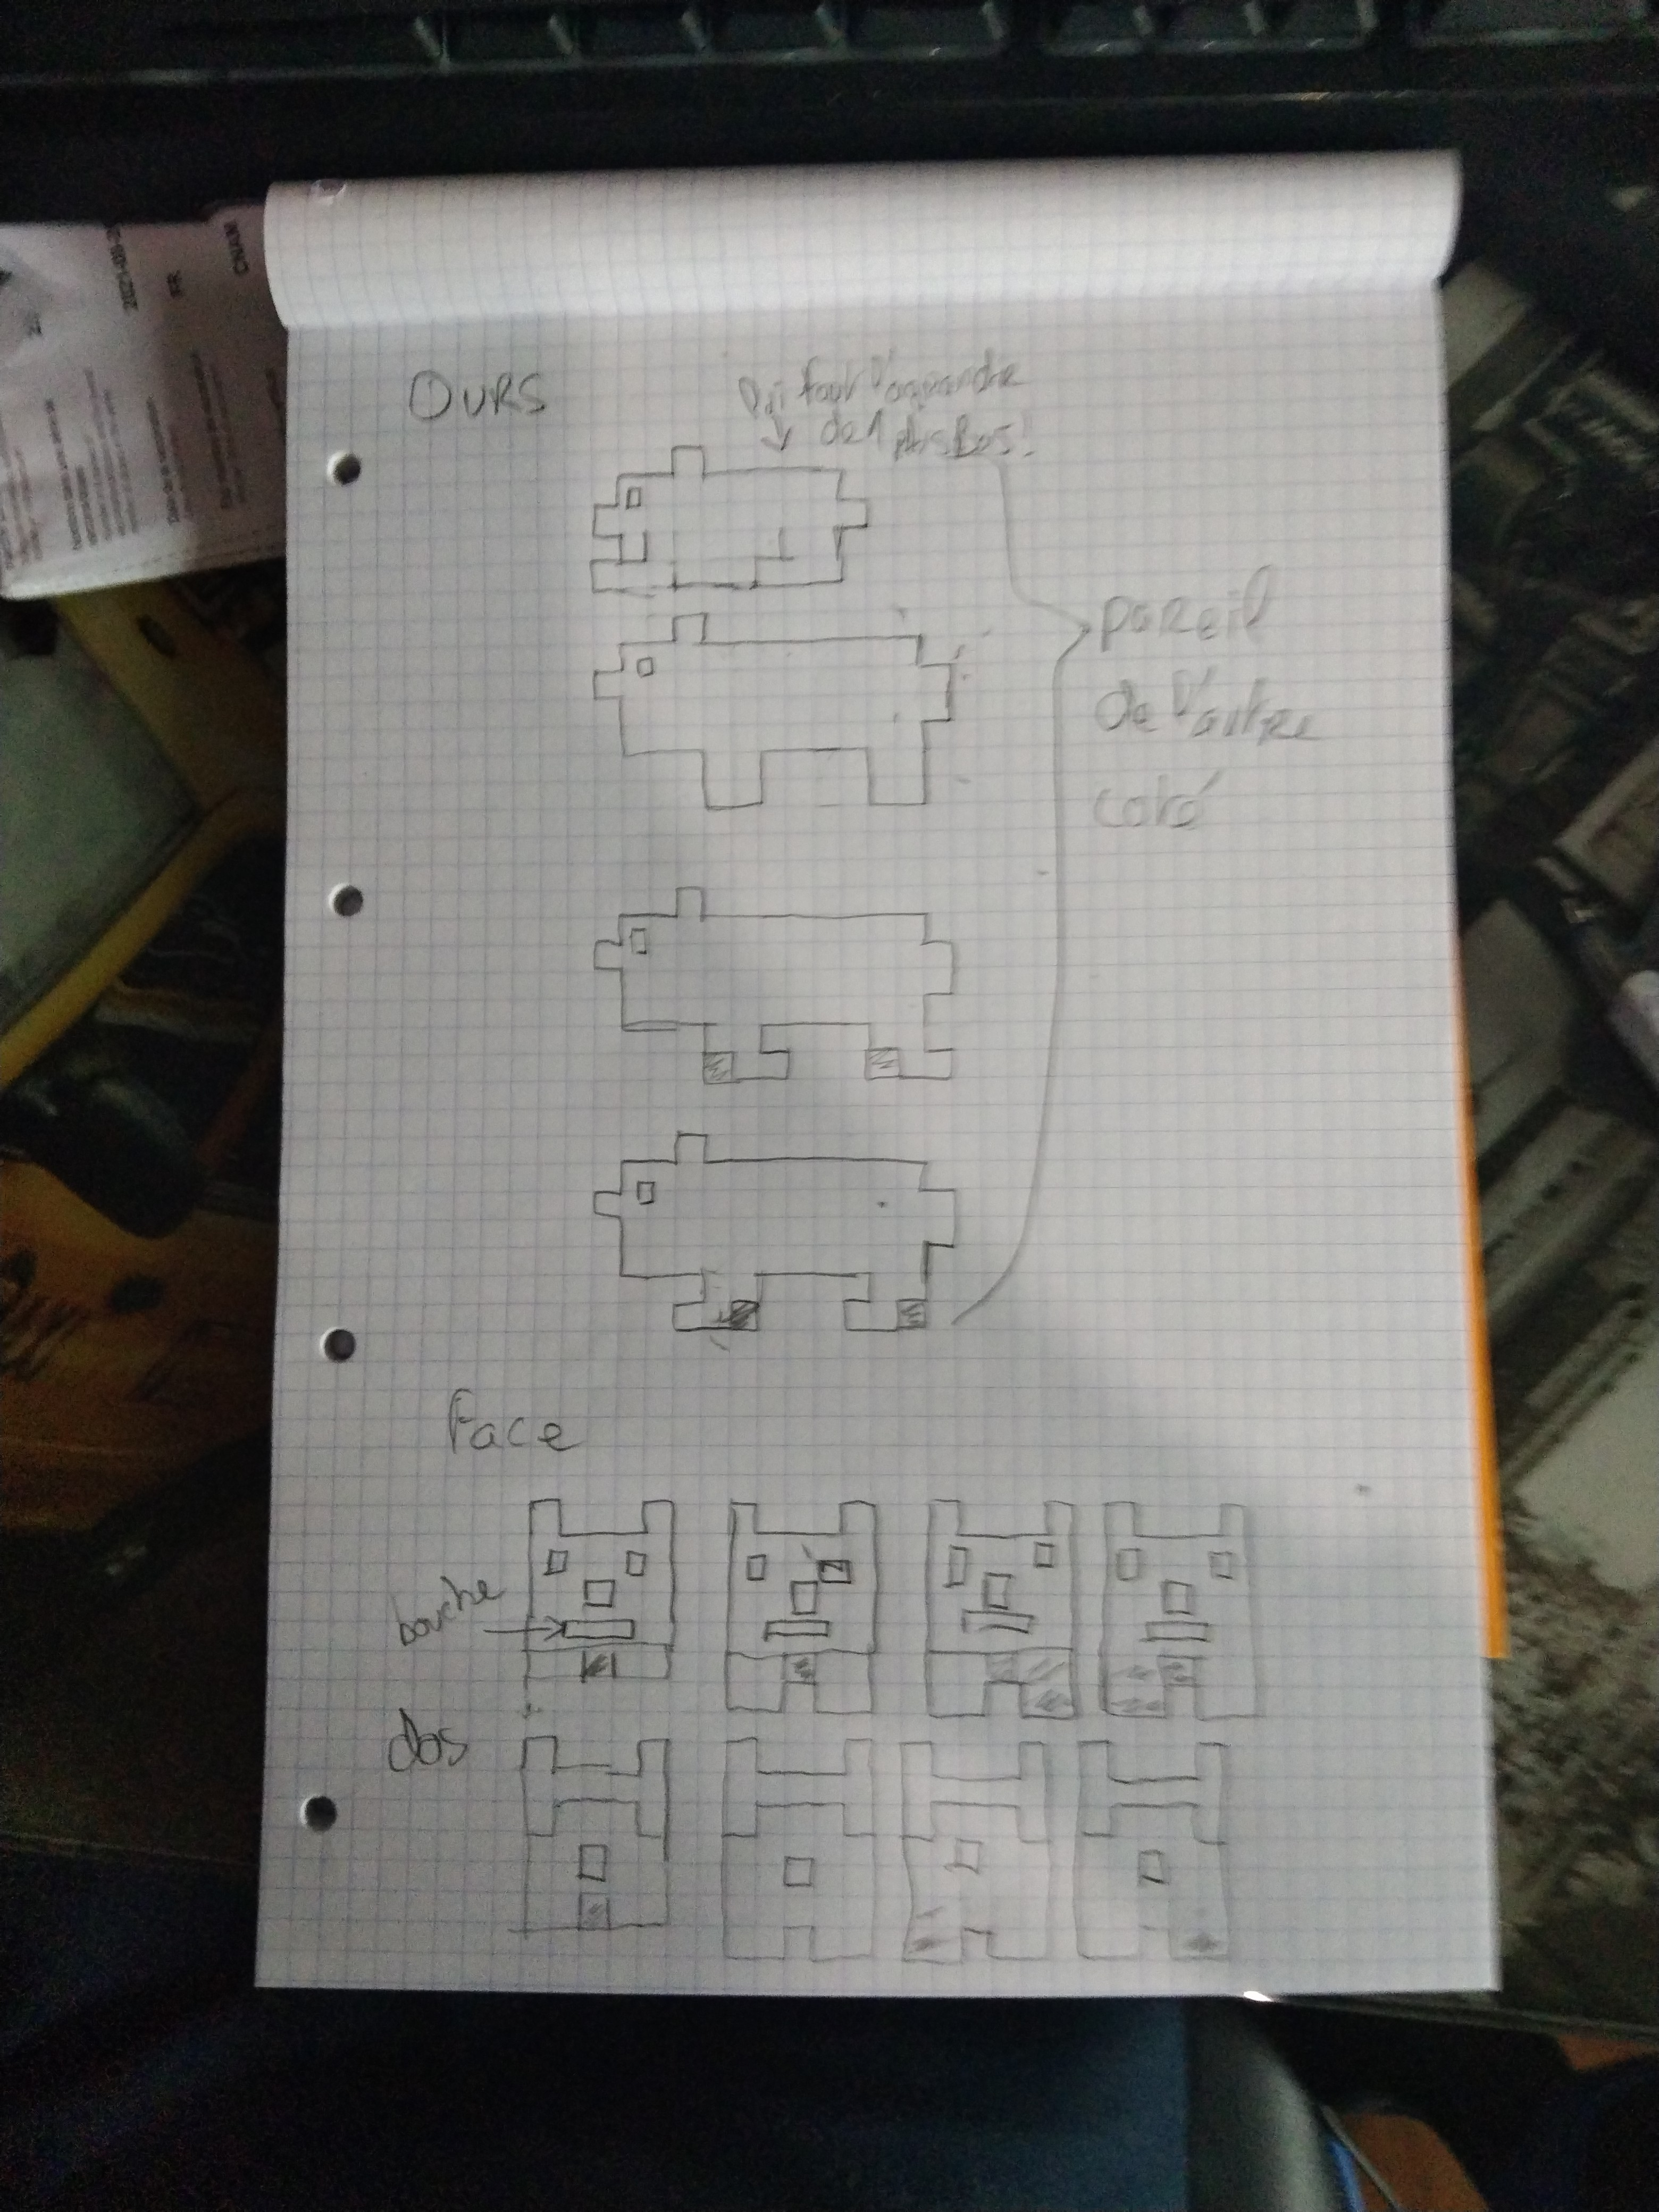
\includegraphics[width=0.5\linewidth]{images/ours.jpg}
 \caption{croquis de l'ours}
 \label{fig::example::one}
\end{figure*}
\\
\begin{figure*}[ht!]
 \centering
 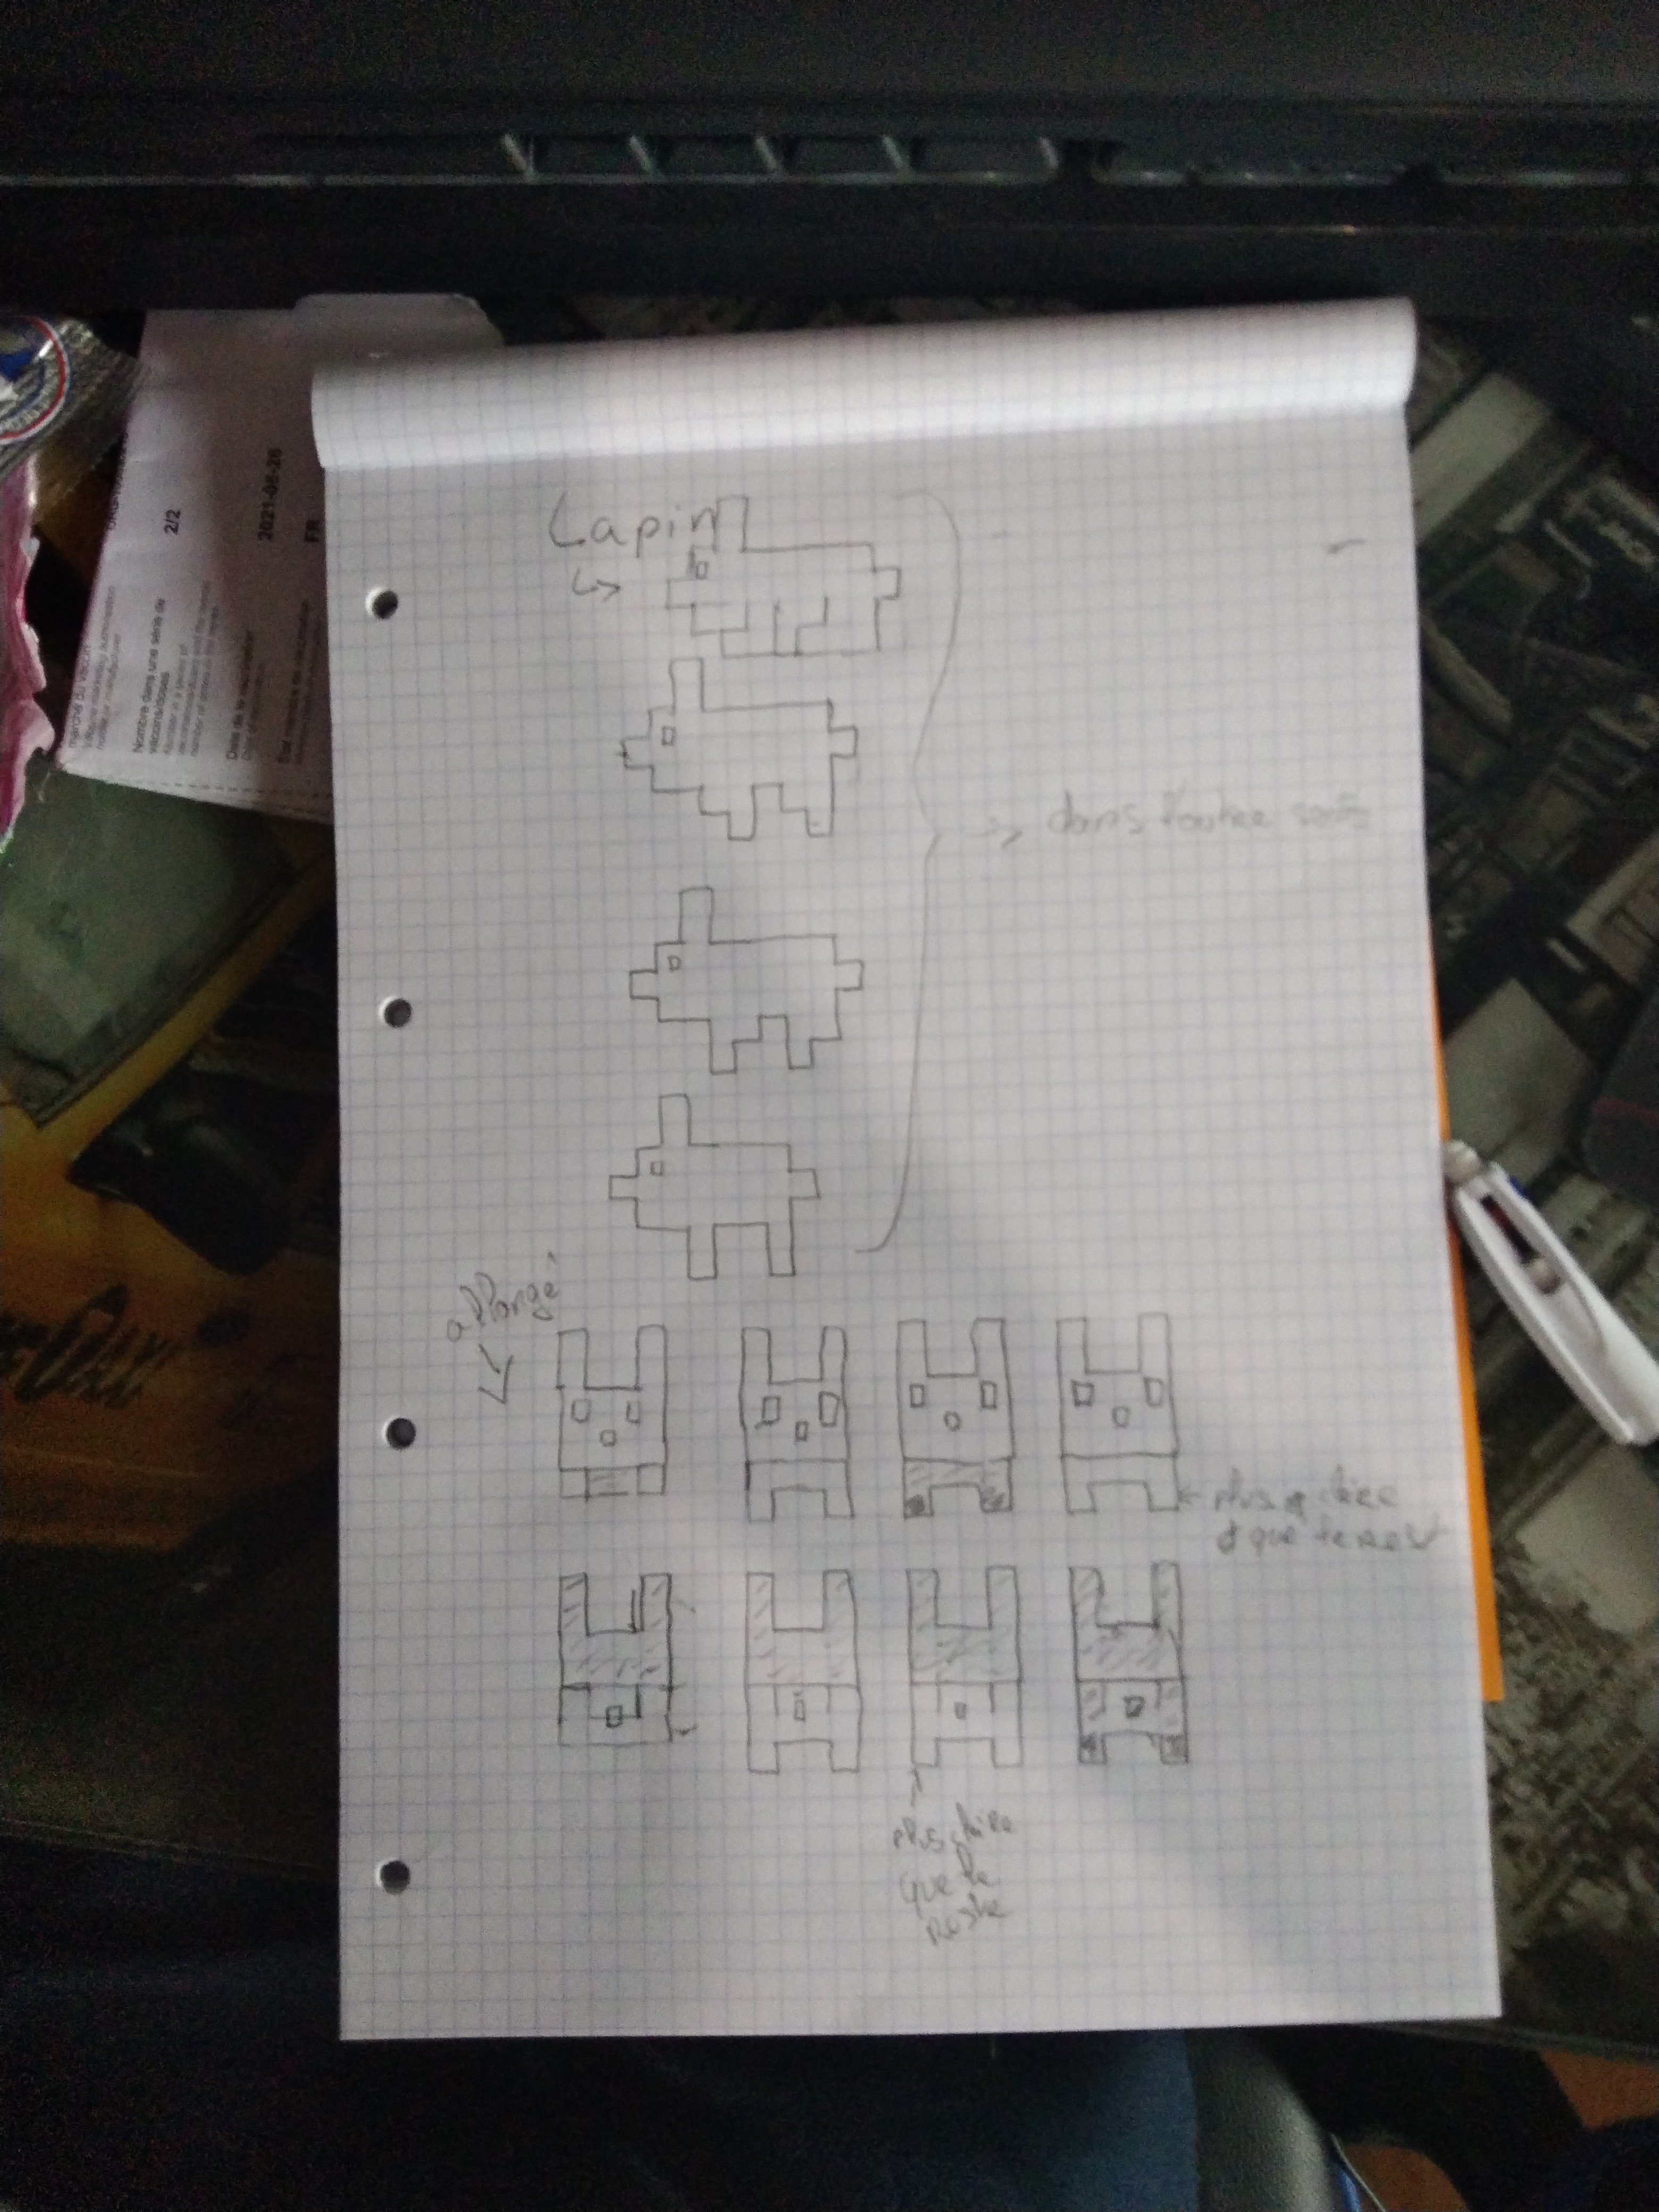
\includegraphics[width=0.5\linewidth]{images/lapin.jpg}
 \caption{croquis du lapin}
 \label{fig::example::one}
\end{figure*}
\\
\begin{figure*}[ht!]
 \centering
 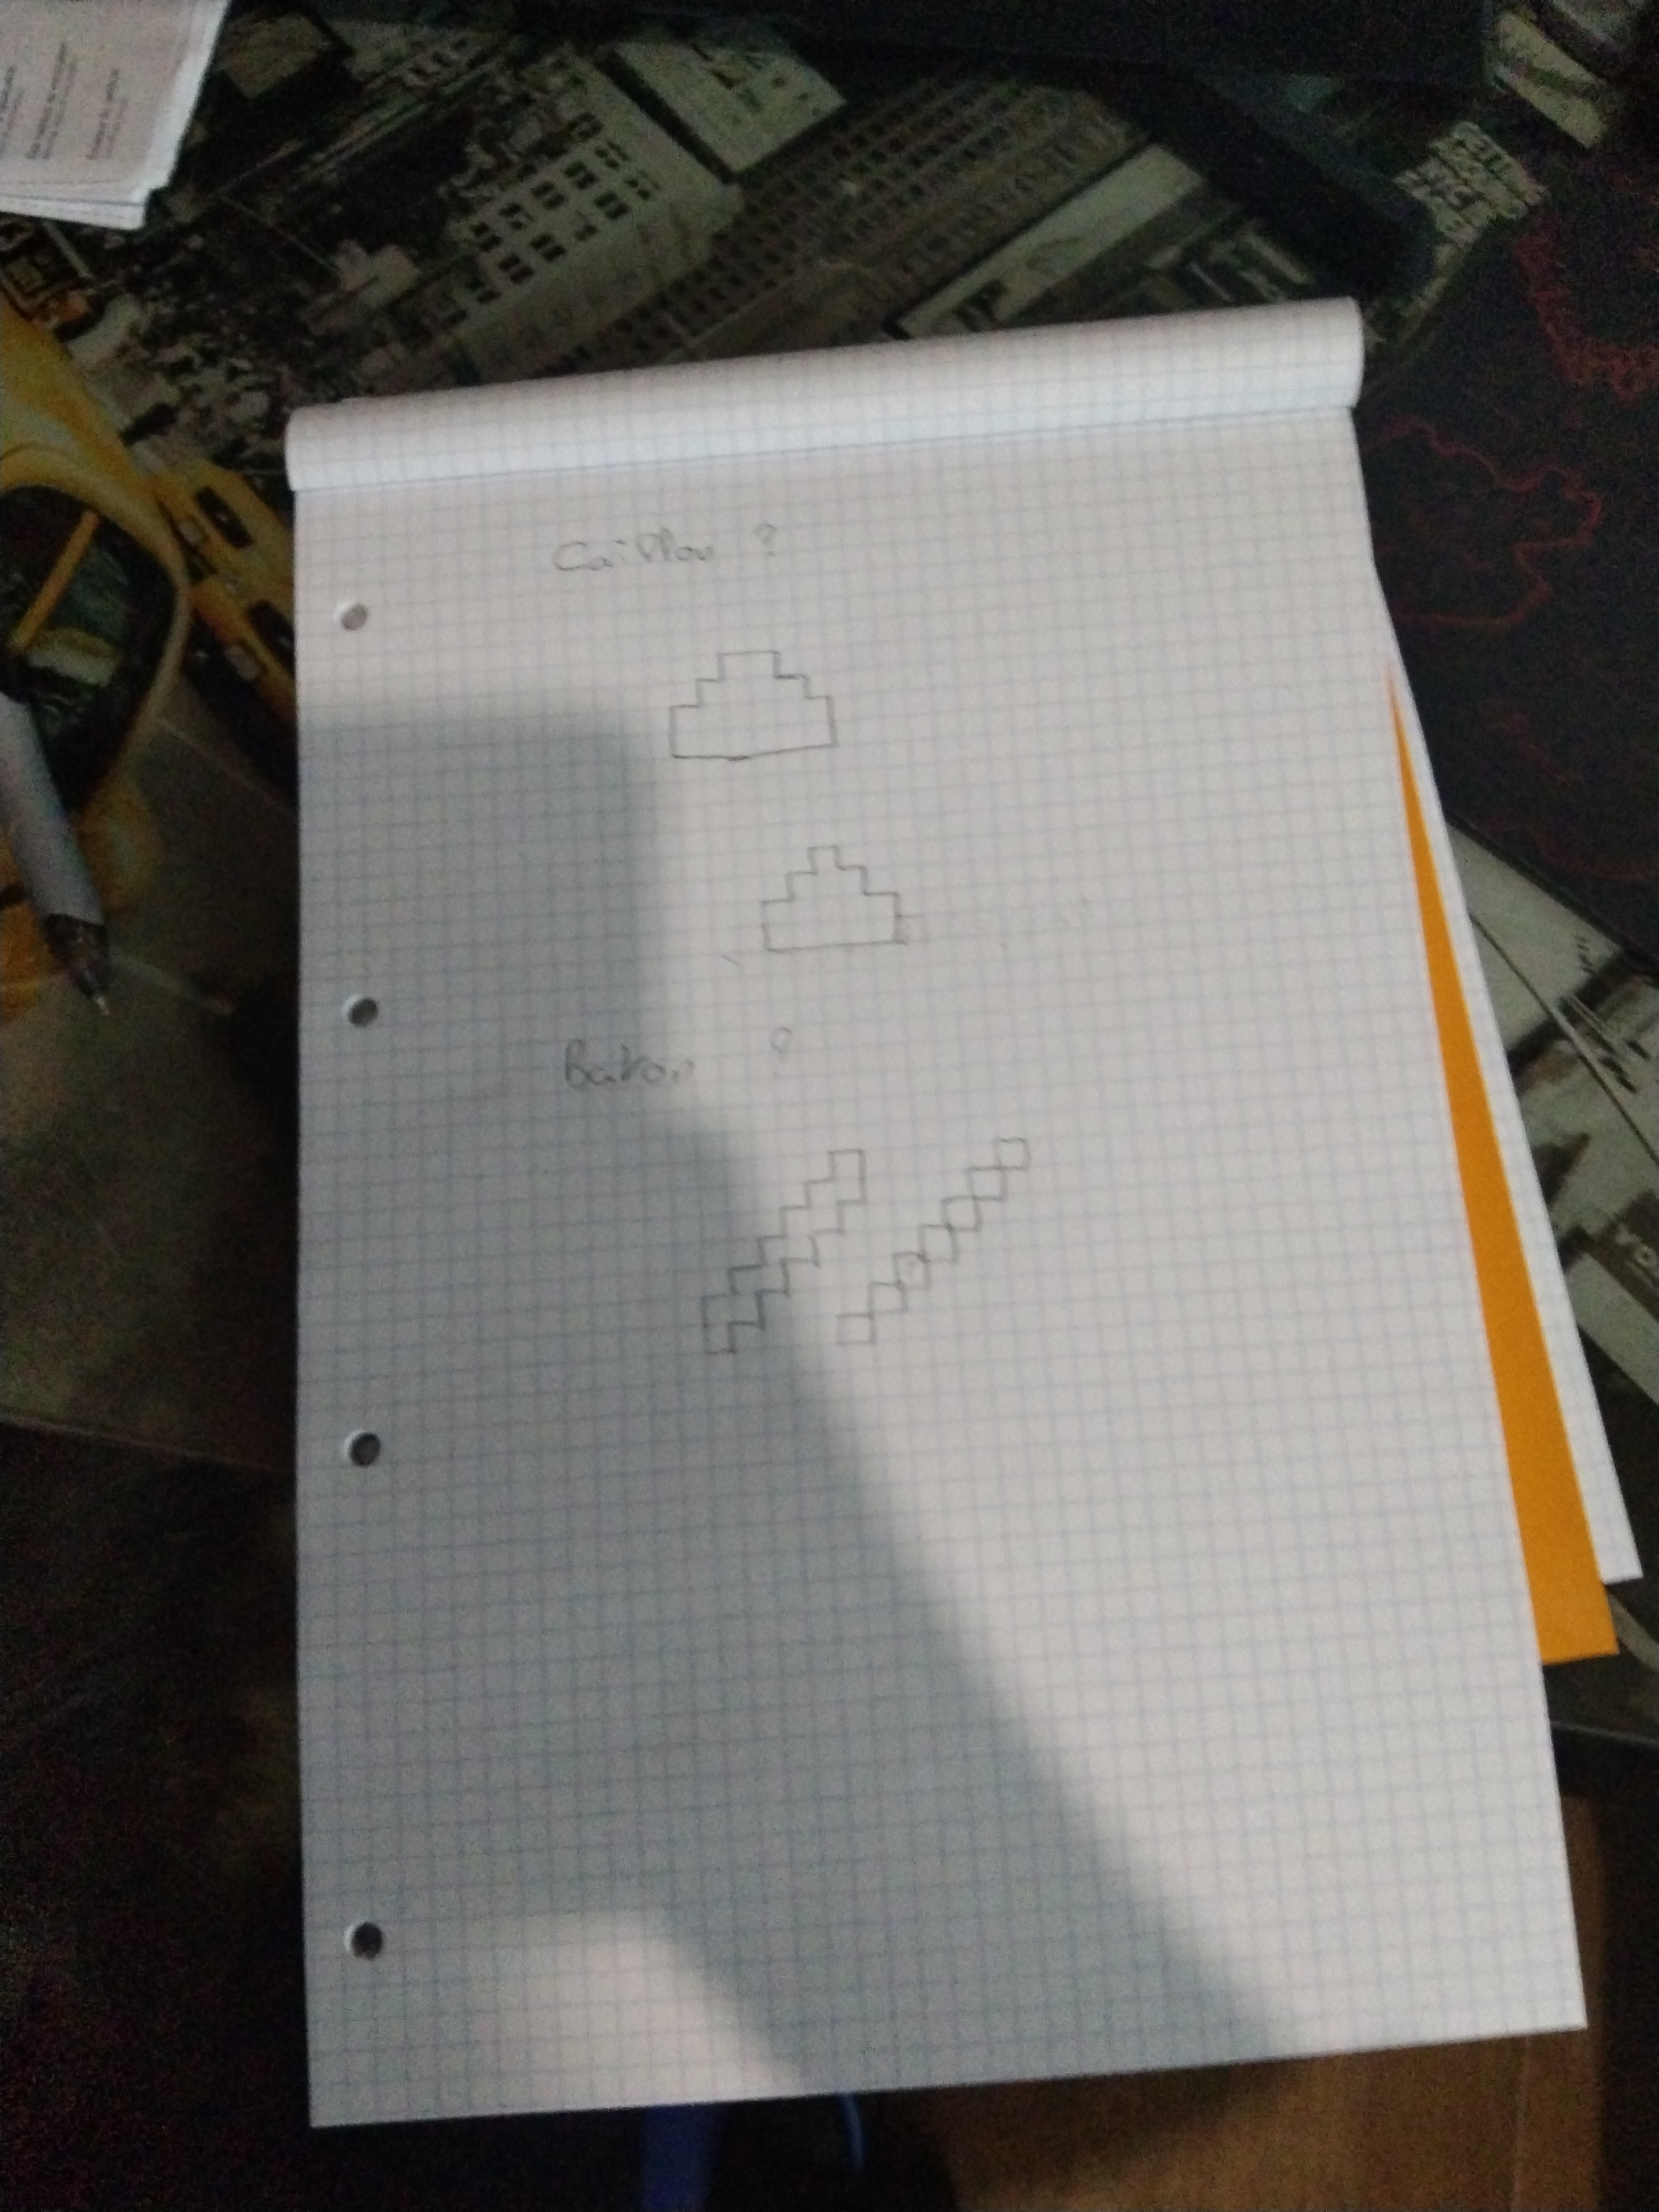
\includegraphics[width=0.5\linewidth]{images/caillou&batton}
 \caption{croquis du caillou et du baton}
 \label{fig::example::one}
\end{figure*}
\\
\newpage
{\color{white}jeejej}
\newpage
\item Et ensuite il a donc fait les sprites de chaque entités en croquis :
\\
\begin{figure*}[ht!]
 \centering
 
\includegraphics[width=0.5\linewidth]{images/loup.png}
 \caption{sprite du loup}
 \label{fig::example::one}
\end{figure*}
\\
\begin{figure*}[ht!]
 \centering
 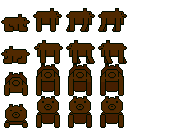
\includegraphics[width=0.5\linewidth]{images/ours.png}
 \caption{sprite de l'ours}
 \label{fig::example::one}
\end{figure*}
\\
\begin{figure*}[ht!]
  \begin{minipage}[c]{.5\linewidth}
   \centering
   
\includegraphics[width=\linewidth]{images/caillou.png}
  \end{minipage} \hfill
  \begin{minipage}[c]{.5\linewidth}
   \centering
   
\includegraphics[width=\linewidth]{images/baton.png}
  \end{minipage}
  \caption{(a) sprite du caillou ; (b) sprite du baton}
  \label{fig::example::two}
\end{figure*}
\newpage
\item Il était sur une moyenne de 5-6 heures par sprites par jour, mais il a réparti cela sur plusieurs semaines environ 3-4.\\
\\
\item Ensuite durant un peu plus d'un mois il a fait la fenêtre de menu du jeu sur une moyenne de 4 heures par semaines.\\
\\
\item a passer même pas  minutes a faire le sprite de l'herbe :\\
\begin{figure*}[ht!]
 \centering
 
\includegraphics[width=0.3\linewidth]{images/herbe.png}
 \caption{sprite de l'herbe}
 \label{fig::example::one}
\end{figure*}
\\
\item Et enfin il a commencé le Latex le "28 mars 2022" et je l'ai fini le " ".\\
\end{enumerate}
\newpage

\section{Les difficultés rencontrées}

Nous avons eu quelques difficultés sur : \\

\newpage

\section{Les éventuels ajout qu'on aurait voulu}

Si nous aurions eu plus de temps nous aurions voulu faire des fins alternatives et d'autres fenêtres comme une fenêtre de paramètres.\\

\newpage

\section{Les éventuels sources}

Pour les sprites : \\
		 Sprite de l'humain : nous n'avons pas trouver de sources.\\
		 Sprite de l'orc : C'est une recoloration du sprite de l'humain.\\
		 Les autres sprites : Nous n'avons pas de sources puisqu'ils ont étaient fait par nos soins.\\
Pour la texture de la map : \\
Pour "l'algorithme" : \\
Pour le code : \\

\newpage

\section{Conclusion}

Pour conclure nous aurions aimaient / voulu :\\

\newpage
\end{document}
